\documentclass[twoside,11pt]{article}

% JMLR Machine Learning Open Source Software (MLOSS) track: at most four pages
% excluding references. Style file shared with the full paper (../jmlr2e.sty).
\usepackage[abbrvbib,preprint]{../jmlr2e}

\usepackage[T1]{fontenc}
\usepackage{lmodern}
\usepackage{microtype}
\usepackage{amsmath}
\usepackage{booktabs}
\usepackage{xcolor}
\usepackage{enumitem}
\usepackage{tikz}
\usetikzlibrary{arrows.meta,positioning,fit,backgrounds,calc}
\usepackage{lastpage}

\setlist{itemsep=1pt,topsep=2pt}
\setlength{\emergencystretch}{3em}

\definecolor{accent}{HTML}{c0602a}
\definecolor{soft}{HTML}{eef2f5}
\definecolor{tfm}{HTML}{2f6f8f}
\definecolor{ctwo}{HTML}{9b4f7f}
\definecolor{sun}{HTML}{3d7f5a}

\newcommand{\repourl}{https://github.com/DanK10097110/TSFM-Interp}
\newcommand{\tool}{\textsc{TSFM-Lens}}

\jmlrheading{}{2026}{1-\pageref{LastPage}}{}{}{}{Dan Kushnir}
\ShortHeadings{TSFM-Lens: Comparative Interpretability of TSFMs}{Kushnir}
\firstpageno{1}

\begin{document}

\title{\tool: A Python Toolkit for Controlled, Causal and\\ Confirmatory Interpretability of Time-Series Foundation Models}

\author{\name Dan Kushnir \email dan.kushnir@spialert.com}

\editor{}

\maketitle

\begin{abstract}%
\tool{} is an open-source Python toolkit that turns a list of time-series foundation model (TSFM)
checkpoints into a single self-contained interpretability report with one command. It compares models
with different architectures on a measured common time axis, validates every probe on a synthetic
benchmark with exact generative ground truth, defines concepts by their causal effect on the forecast
against matched random nulls, and tests exploratory claims once on a sealed held-out split. Every
reported number carries an evidence class and a plain-language explanation. The toolkit ships adapters
for TimesFM, the Chronos family, Sundial, Timer and Lag-Llama, a zero-code adapter for Hugging Face
checkpoints, a complete example run and a test suite of over two thousand tests. It is released under the
MIT license at \url{\repourl}.
\end{abstract}

\begin{keywords}
  interpretability, time-series foundation models, sparse autoencoders, causal intervention, open-source software
\end{keywords}

\section{Introduction}

Pretrained forecasters such as TimesFM \citep{das2024timesfm}, Chronos \citep{ansari2024chronos,
ansari2025chronos2}, Sundial \citep{liu2025sundial} and Timer \citep{liu2024timer} are used zero-shot, yet
little is known about what they compute. Libraries such as TransformerLens \citep{nanda2022transformerlens},
pyvene \citep{wu2024pyvene}, nnsight \citep{fiottokaufman2025nnsight} and SAELens \citep{bloom2024saelens}
provide hooks, patching and sparse dictionaries for one model at a time. Three properties of TSFMs make a
direct transfer unreliable: tokens cover 1 to 96 time steps depending on the architecture, so positions are
not comparable across models; real series carry no labels for trend, seasonality or noise, so probes cannot
be checked; and the causal effects of internal features are small enough that an uncontrolled measurement
yields a confident false positive. \tool{} is built around these problems. It is a \emph{comparative} tool:
its unit of analysis is a panel of models on a shared benchmark, and its output is a report that a
non-specialist can read and an expert can audit.

\section{Architecture}

The repository contains two separately installable packages (Figure~\ref{fig:arch}).
\texttt{tsfm\_benchmark} builds and validates corpora; \texttt{tsfm\_lens} analyzes models and renders the
report. Their dependencies overlap only in NumPy, SciPy and PyYAML, so the benchmark can be used on its own.

\begin{figure}[t]
\centering
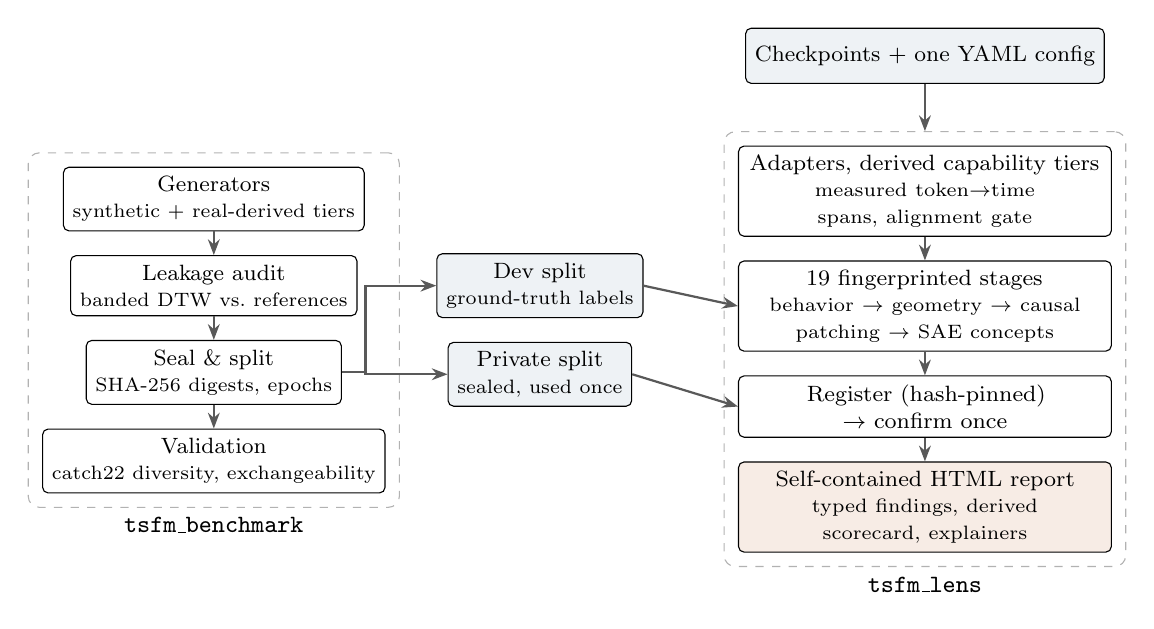
\begin{tikzpicture}[
  node distance=3mm and 6mm,
  box/.style={draw, rounded corners=2pt, align=center, font=\footnotesize, minimum height=7mm, fill=white},
  pkg/.style={draw=gray!60, dashed, rounded corners=4pt, inner sep=5pt},
  arr/.style={-{Stealth[length=2mm]}, thick, gray!70!black}]
  \node[box] (gen) {Generators\\{\scriptsize synthetic + real-derived tiers}};
  \node[box, below=of gen] (aud) {Leakage audit\\{\scriptsize banded DTW vs.\ references}};
  \node[box, below=of aud] (seal) {Seal \& split\\{\scriptsize SHA-256 digests, epochs}};
  \node[box, below=of seal] (val) {Validation\\{\scriptsize catch22 diversity, exchangeability}};
  \draw[arr] (gen) -- (aud); \draw[arr] (aud) -- (seal); \draw[arr] (seal) -- (val);
  \begin{scope}[on background layer]
    \node[pkg, fit=(gen)(val), label={[font=\small\bfseries]below:\texttt{tsfm\_benchmark}}] {};
  \end{scope}
  \node[box, right=10mm of aud, fill=soft] (dev) {Dev split\\{\scriptsize ground-truth labels}};
  \node[box, below=of dev, fill=soft] (priv) {Private split\\{\scriptsize sealed, used once}};
  \draw[arr] (seal.east) -- ++(3mm,0) |- (dev.west);
  \draw[arr] (seal.east) -- ++(3mm,0) |- (priv.west);
  \node[box, right=12mm of dev, yshift=12mm, text width=45mm] (ad) {Adapters, derived capability tiers\\{\scriptsize measured token$\to$time spans, alignment gate}};
  \node[box, below=of ad, text width=45mm] (st) {19 fingerprinted stages\\{\scriptsize behavior $\to$ geometry $\to$ causal patching $\to$ SAE concepts}};
  \node[box, below=of st, text width=45mm] (reg) {Register (hash-pinned) $\to$ confirm once};
  \node[box, below=of reg, text width=45mm, fill=accent!12] (rep) {Self-contained HTML report\\{\scriptsize typed findings, derived scorecard, explainers}};
  \draw[arr] (ad) -- (st); \draw[arr] (st) -- (reg); \draw[arr] (reg) -- (rep);
  \begin{scope}[on background layer]
    \node[pkg, fit=(ad)(rep), label={[font=\small\bfseries]below:\texttt{tsfm\_lens}}] (lens) {};
  \end{scope}
  \draw[arr] (dev.east) -- (st.west);
  \draw[arr] (priv.east) -- (reg.west);
  \node[box, above=6mm of lens.north, fill=soft] (ck) {Checkpoints + one YAML config};
  \draw[arr] (ck) -- (lens.north);
\end{tikzpicture}
\caption{Architecture of \tool{}. The benchmark package produces leakage-audited, sealed corpora with exact
ground truth. The analysis package loads each checkpoint through an adapter, runs a gated stage pipeline on
the dev split, confirms registered claims once on the private split and renders one report.}
\label{fig:arch}
\end{figure}

\paragraph{Benchmark.} Generators come in two labeled tiers: a \emph{synthetic} tier (additive parametric
series and frozen archetypes) that touches no real data and records every generative component, and a
\emph{real-derived} tier (mixtures, block bootstrap, sequential synthesis) with attributional ground truth.
Every sample passes a leakage audit against real reference archives; dev and private splits come from
disjoint seed ranges, are hashed, and can be re-minted as fresh epochs. A validation module measures diversity
in catch22 feature space and tests dev/private exchangeability. Structured corruptions and single-knob
generator counterfactuals provide controlled perturbations with known effects.

\paragraph{Adapters.} A model is wrapped by an adapter that exposes loading, prediction, the module and token
time spans. Its capability tier (black box, observable, steerable, decomposable) is \emph{derived} from the
methods it implements, and stages that need a higher tier are skipped with the reason rendered in the report.
A zero-code adapter discovers layers and \emph{measures} token spans from impulse responses for Hugging Face
checkpoints, refusing rather than guessing; hand-written adapters start from a template, and a single command
(\texttt{-{}-check-adapter}) runs conformance, reach and alignment checks.

\paragraph{Alignment and stages.} Tokens are overlap-pooled onto common time windows, so every cross-model
statistic compares the same stretch of time; an alignment gate verifies this per layer during extraction. The
pipeline has 19 stages grouped by the evidence they can produce: behavioral (accuracy, calibration, cost, tokenizer
checks), descriptive (effective dimension, logit-lens style depth profiles), geometric and linear-translatable
(CKA, RSA, stitching gain over an input baseline), causal within-model (corruption fingerprints, activation
patching, head ablation) and concept-level (TopK sparse autoencoders, a feature ablation battery, cross-model
concept matching). Each stage declares the configuration keys it depends on; these are fingerprinted, so cached
artifacts are reused only when still valid.

\paragraph{Causal concepts.} A sparse-dictionary feature counts as causal only if removing it changes a forecast
channel (level, trend, seasonality, shape, accuracy, \dots) more than removing a random direction of matched size
on the same series, after reach controls confirm that the intervention lands (self-patch exactly zero,
cross-patch nonzero). Causal features are clustered into concepts within and across models, and sharing is tested
at two levels: whether two models' concepts select the \emph{same inputs}, and whether they have the \emph{same
effect on those inputs}, each against its own null.

\paragraph{Statistics and confirmation.} All intervals and $p$-values resample series rather than windows. Every
test belongs to a named correction family, and a multiplicity ledger flags families whose smallest attainable
adjusted $p$-value cannot reach the significance level. Exploratory claims are frozen in a hash-pinned registry
and tested once on the sealed split; a repeated look is recorded.

\paragraph{Report.} The output is one HTML file without external dependencies. Sections pose plain questions
(``Is the comparison fair?'', ``What causally drives the forecast?''), every figure carries a caption and an
expandable explanation of how to read it and what it cannot show, the scorecard is derived from artifacts by
explicit rules with no model names hard-coded, and every claim is a typed record with an evidence class and a
generated caveat. Skipped or failed sections render visibly with their reason.

\section{Usage}

After \texttt{pip install -e . \&\& pip install -e tsfm\_lens}, a full analysis is
\begin{center}\texttt{python run.py -{}-config configs/examples/large\_4model.yaml}\end{center}
Presets cover a CPU-only smoke test with mock models (minutes), a single model and a pair. The CLI also offers
a preflight check (\texttt{-{}-doctor}), partial reruns (\texttt{-{}-stages}, \texttt{-{}-force}), alignment and
adapter checks for new checkpoints, and a provenance diff between a run's recorded environment and the current
one. New report sections, claims and configuration fields plug into declared interfaces that keep the fingerprints
and evidence classes consistent.

\paragraph{Example.} The repository includes a complete run on TimesFM~2.5, Chronos-2, Sundial and Chronos-Bolt
(\texttt{examples/concept\_atlas\_v2}: report, configuration and per-stage artifacts; 6.4 hours on one 24~GB
GPU). In it, 293 sparse features clear their causal nulls, mostly acting on forecast level and shape; the models
agree on which inputs a concept groups (20 of 20 registered claims confirmed on 800 sealed series) but rarely on
what it does to them. A curated ledger (\texttt{FINDINGS.md}) records every result, positive and negative, with
its evidence class and reproduction command, including cases where a built-in control overturned a plausible but
wrong result.

\section{Quality and Availability}

The code is released under the MIT license. The test suite (over 2{,}100 tests for \texttt{tsfm\_lens}, plus
golden-hash regeneration tests for the benchmark) runs in continuous integration on mock adapters, against
pinned dependencies and, weekly, against the latest releases of the load-bearing libraries. Tests follow a
planted-answer standard: each load-bearing assertion must be shown to fail against a deliberately planted
regression. Documentation includes a README, a guide to adding models with a pitfall checklist, a worked report
walkthrough, and stage, adapter and glossary documentation generated from the code (with
a \texttt{-{}-check} mode that detects drift). Exact
dependency pins and the reason for each are recorded in \texttt{DEPENDENCIES.md}, and every run records its
environment. \tool{} is univariate by design, captures only the parts of a model an adapter exposes, and relies on
synthetic ground truth whose generators encode assumptions about which structure matters; the report states these
limits alongside the results they qualify.

\vskip 0.2in
\bibliography{../references}

\end{document}
